\documentclass{article}
\usepackage{amsmath}
\usepackage{amssymb}
\usepackage{amsthm}
\usepackage{listings}
\usepackage{xcolor}
\usepackage{graphicx}

\definecolor{codegreen}{rgb}{0,0.6,0}
\definecolor{codegray}{rgb}{0.5,0.5,0.5}
\definecolor{codepurple}{rgb}{0.58,0,0.82}
\definecolor{backcolour}{rgb}{0.95,0.95,0.92}

\lstdefinestyle{mystyle}{
    backgroundcolor=\color{backcolour},   
    commentstyle=\color{codegreen},
    keywordstyle=\color{magenta},
    numberstyle=\tiny\color{codegray},
    stringstyle=\color{codepurple},
    basicstyle=\ttfamily\footnotesize,
    breakatwhitespace=false,         
    breaklines=true,                 
    captionpos=b,                    
    keepspaces=true,                 
    numbers=left,                    
    numbersep=5pt,                  
    showspaces=false,                
    showstringspaces=false,
    showtabs=false,                  
    tabsize=4,
    language=Python
}
\lstset{style=mystyle}

\title{EEE 554 Homework 4}
\author{Chaofei Guo (Student ID: 1237382330, ASURITE: chaofeig)}
\date{}

\begin{document}

\maketitle

\section*{Problem 1}
\textbf{Problem Statement:}
The random variable $x$ has the Erlang density $f(x) \sim c^4 x^3 e^{-cx} U(x)$. We observe the samples $x_i = 3.1, 3.4, 3.3$. Find the ML estimate $\hat{c}$ of $c$.

\begin{proof}[Solution]
	The probability density function for the Erlang random variable is $f(x, c) = \frac{c^4}{3!} x^3 e^{-cx}$. For $n$ independent samples, the likelihood function is:
	\[ f(X, c) = \prod_{i=1}^n \frac{c^4}{6} x_i^3 e^{-cx_i} = \left( \frac{c^4}{6} \right)^n \left( \prod_{i=1}^n x_i^3 \right) e^{-c \sum_{i=1}^n x_i} \]
	The log-likelihood function $L(c)$ is:
	\[ L(c) = n(4\ln c - \ln 6) + 3 \sum_{i=1}^n \ln x_i - c \sum_{i=1}^n x_i \]
	Setting the derivative with respect to $c$ to zero for the maximum:
	\[ \frac{dL(c)}{dc} = \frac{4n}{c} - \sum_{i=1}^n x_i = 0 \implies \hat{c} = \frac{4n}{\sum_{i=1}^n x_i} \]
	Given the samples $3.1, 3.4, 3.3$, we have $n=3$ and a sum of $9.8$. Substituting these values:
	\[ \hat{c} = \frac{4(3)}{9.8} = \frac{12}{9.8} \approx 1.2245 \]
	The ML estimate $\hat{c}$ is approximately $1.2245$.
\end{proof}


\section*{Problem 2}
\textbf{Problem Statement:}
The random variable $x$ has the truncated exponential density $f(x) = ce^{-c(x-x_0)} U(x-x_0)$. Find the ML estimate $\hat{c}$ of $c$ in terms of the $n$ samples $x_i$ of $x$.

\begin{proof}[Solution]
	For $n$ independent and identically distributed samples, the likelihood function is:
	\[ f(X, c) = \prod_{i=1}^n c e^{-c(x_i - x_0)} = c^n e^{-c \sum_{i=1}^n (x_i - x_0)} \]
	The log-likelihood function is:
	\[ L(c) = n \ln c - c \sum_{i=1}^n (x_i - x_0) \]
	Differentiating with respect to $c$ and setting it to zero:
	\[ \frac{dL(c)}{dc} = \frac{n}{c} - \sum_{i=1}^n (x_i - x_0) = 0 \]
	Solving for $c$ yields the ML estimate:
	\[ \hat{c} = \frac{n}{\sum_{i=1}^n (x_i - x_0)} = \frac{1}{\overline{x} - x_0} \]
	where $\overline{x}$ is the sample mean.
\end{proof}


\section*{Problem 3}
\textbf{Problem Statement:}
Show that if $L(x, \theta) = \log f(x, \theta)$ is the likelihood function of a random variable $x$, then:
\[ E \left\{ \left| \frac{\partial L(x, \theta)}{\partial \theta} \right|^2 \right\} = -E \left\{ \frac{\partial^2 L(x, \theta)}{\partial \theta^2} \right\} \]

\begin{proof}[Solution]
	Starting from the normalization condition $\int f(x, \theta) dx = 1$, we differentiate with respect to $\theta$:
	\[ \int \frac{\partial f(x, \theta)}{\partial \theta} dx = 0 \]
	Using the identity $\frac{\partial L}{\partial \theta} = \frac{1}{f} \frac{\partial f}{\partial \theta}$, we have $\frac{\partial f}{\partial \theta} = f \frac{\partial L}{\partial \theta}$. Thus:
	\[ \int f \frac{\partial L}{\partial \theta} dx = E \left\{ \frac{\partial L}{\partial \theta} \right\} = 0 \]
	Differentiating the integral $\int \frac{\partial f}{\partial \theta} dx = 0$ a second time:
	\[ \int \frac{\partial^2 f(x, \theta)}{\partial \theta^2} dx = 0 \]
	The second derivative of $L$ is given by:
	\[ \frac{\partial^2 L}{\partial \theta^2} = \frac{\partial}{\partial \theta} \left( \frac{1}{f} \frac{\partial f}{\partial \theta} \right) = \frac{1}{f} \frac{\partial^2 f}{\partial \theta^2} - \frac{1}{f^2} \left( \frac{\partial f}{\partial \theta} \right)^2 = \frac{1}{f} \frac{\partial^2 f}{\partial \theta^2} - \left( \frac{\partial L}{\partial \theta} \right)^2 \]
	Taking the expectation:
	\[ E \left\{ \frac{\partial^2 L}{\partial \theta^2} \right\} = \int f \left[ \frac{1}{f} \frac{\partial^2 f}{\partial \theta^2} - \left( \frac{\partial L}{\partial \theta} \right)^2 \right] dx = \int \frac{\partial^2 f}{\partial \theta^2} dx - E \left\{ \left| \frac{\partial L}{\partial \theta} \right|^2 \right\} \]
	Since $\int \frac{\partial^2 f}{\partial \theta^2} dx = 0$, the relationship simplifies to:
	\[ E \left\{ \frac{\partial^2 L}{\partial \theta^2} \right\} = -E \left\{ \left| \frac{\partial L}{\partial \theta} \right|^2 \right\} \]
	Multiplying by $-1$ completes the proof.
\end{proof}


\section*{Problem 4}
\textbf{Problem Statement:}
A complex discrete-time WSS process $z(\cdot)$ has mean zero and spectral density $S_z$. A new process $w(\cdot)$ is defined by $w(k) = z(k)e^{i\theta}$ where $\theta \sim U[0, 2\pi]$ is independent of $z(\cdot)$. Show that $S_w(\omega) = S_z(\omega)$ for all $\omega$.

\begin{proof}[Solution]
	To show that $S_w(\omega) = S_z(\omega)$, we first verify that the process $w(k)$ is Wide-Sense Stationary (WSS) and then calculate its spectral density.
	
	\textbf{1. Mean of $w(k)$}\\
	The mean of $w(k)$ is given by:
	\[ \mu_w(k) = E[w(k)] = E[z(k)e^{i\theta}] \]
	Since $z(\cdot)$ and $\theta$ are independent, the expectation of their product is the product of their expectations:
	\[ \mu_w(k) = E[z(k)] E[e^{i\theta}] \]
	Given that $z(\cdot)$ has mean zero ($\mu_z = 0$), we have:
	\[ \mu_w(k) = 0 \cdot E[e^{i\theta}] = 0 \]
	Thus, $\mu_w$ is constant and equal to zero.
	
	\textbf{2. Autocovariance of $w(k)$}\\
	The autocovariance of $w(k)$ for lag $m$ is defined as:
	\[ C_w(k, k+m) = E[w(k)w^*(k+m)] - E[w(k)]E[w^*(k+m)] \]
	Since the mean is zero, this simplifies to the autocorrelation:
	\[ C_w(k, k+m) = E[(z(k)e^{i\theta})(z(k+m)e^{i\theta})^*] \]
	\[ C_w(k, k+m) = E[z(k)z^*(k+m) e^{i\theta}e^{-i\theta}] \]
	\[ C_w(k, k+m) = E[z(k)z^*(k+m) \cdot 1] \]
	By independence:
	\[ C_w(k, k+m) = E[z(k)z^*(k+m)] \]
	Because $z(\cdot)$ is WSS, its autocovariance depends only on the lag $m = (k+m) - k$
	\[ C_w(m) = C_z(m) \]
	
	\textbf{3. Spectral Density}\\
	The spectral density $S_w(\omega)$ is defined as the Discrete-Time Fourier Transform (DTFT) of the autocovariance function $C_w(m)$
	\[ S_w(\omega) = \sum_{m=-\infty}^{\infty} C_w(m) e^{-i\omega m} \]
	Substituting $C_w(m) = C_z(m)$ into the definition:
	\[ S_w(\omega) = \sum_{m=-\infty}^{\omega} C_z(m) e^{-i\omega m} = S_z(\omega) \]
	Therefore, $S_w(\omega) = S_z(\omega)$ for all $\omega$.
\end{proof}


\section*{Problem 5}
\textbf{Problem Statement:}
A discrete-time white process $x(\cdot)$ with variance $\sigma^2$ is passed through a stable discrete-time LTI system with impulse response $h(\cdot)$. Find the variance of the output process $y(\cdot)$ in terms of $\sigma^2$ and $h$.

\begin{proof}[Solution]
	Let $x(k)$ be a white process. Its autocovariance is given by $C_x(k) = \sigma^2 \delta(k)$. The output of the LTI system is $y(k) = \sum_{n} h(n)x(k-n)$.
	
	The variance of the output process is its autocovariance at lag zero, $C_y(0)$. Using the relationship for WSS processes through LTI systems:
	\[ C_y(k) = \sum_{n=-\infty}^{\infty} \sum_{m=-\infty}^{\infty} h(n) h(m) C_x(k-n+m) \]
	Setting $k=0$:
	\[ Var(y) = C_y(0) = \sum_{n} \sum_{m} h(n) h(m) \sigma^2 \delta(m-n) \]
	Due to the sifting property of the Kronecker delta, the sum over $m$ is non-zero only when $m=n$:
	\[ Var(y) = \sigma^2 \sum_{n=-\infty}^{\infty} h(n) h(n) = \sigma^2 \sum_{n=-\infty}^{\infty} |h(n)|^2 \]
	Thus, the output variance is the input variance scaled by the energy of the system's impulse response.
\end{proof}


\section*{Problem 6}
\textbf{Problem Statement:}
A zero-mean WSS discrete-time process $y(\cdot)$ has spectral density:
\[ S_y(\omega) = \frac{5 + 3 \cos(\omega)}{17 + 8 \cos(\omega)} \]
(a) Find the frequency response $H(\omega)$ of a discrete-time LTI system that will produce a process with this spectral density from a unit-variance white input signal $x(\cdot)$.\\
(b) Calculate the autocovariance function $c_y(\kappa)$ for $\kappa \ge 0$.\\
(c) Find the impulse response of a whitening filter for $y(\cdot)$.

\begin{proof}[Solution]
	\textbf{Part (a)}\\
	We use spectral factorization. Given $S_x(\omega) = 1$, we have $S_y(\omega) = |H(\omega)|^2$. Convert to the $z$-domain by letting $e^{j\omega} = z$ and $\cos(\omega) = \frac{1}{2}(z + z^{-1})$:
	\[ S_y(z) = \frac{5 + 1.5(z + z^{-1})}{17 + 4(z + z^{-1})} = \frac{1.5z + 5 + 1.5z^{-1}}{4z + 17 + 4z^{-1}} = \frac{1.5(z+3)(z+1/3)}{4(z+4)(z+1/4)} \]
	To ensure stability and causality, we choose the poles and zeros inside the unit circle ($|z| < 1$):
	\[ S_y(z) = \underbrace{\frac{\sqrt{4.5}(1 + \frac{1}{3}z^{-1})}{4(1 + \frac{1}{4}z^{-1})}}_{H(z)} \cdot \underbrace{\frac{\sqrt{4.5}(1 + \frac{1}{3}z)}{4(1 + \frac{1}{4}z)}}_{H(z^{-1})} \]
	Thus, $H(\omega) = \frac{3}{4\sqrt{2}} \frac{1 + \frac{1}{3}e^{-j\omega}}{1 + \frac{1}{4}e^{-j\omega}}$.
	
	\textbf{Part (b)}\\
	The process is an ARMA(1,1) process defined by $y(k) + \frac{1}{4}y(k-1) = b_0 x(k) + b_1 x(k-1)$ with $b_0 = \frac{3}{4\sqrt{2}}$ and $b_1 = \frac{1}{4\sqrt{2}}$.
	The variance $c_y(0)$ is:
	\[ c_y(0) = \frac{b_0^2 + b_1^2 - 2ab_0b_1}{1-a^2} = \frac{9/32 + 1/32 - 2(1/4)(3/32)}{1 - 1/16} = \frac{17/60}{\text{}} \]
	For $\kappa \ge 1$:
	\[ c_y(1) = b_0 b_1 - a c_y(0) = \frac{3}{32} - \frac{1}{4}\left(\frac{17}{60}\right) = \frac{11}{480} \]
	For $\kappa > 1$, $c_y(\kappa) = (-\frac{1}{4})c_y(\kappa-1)$. Thus:
	\[ c_y(\kappa) = \frac{11}{480} \left( -\frac{1}{4} \right)^{\kappa-1}, \quad \kappa \ge 1 \]

	\textbf{Part (c)}\\
	The whitening filter $H_w(z)$ is the inverse of $H(z)$:
	\[ H_w(z) = \frac{1}{H(z)} = \frac{4\sqrt{2}}{3} \frac{1 + \frac{1}{4}z^{-1}}{1 + \frac{1}{3}z^{-1}} \]
	Performing partial fraction expansion:
	\[ H_w(z) = \frac{4\sqrt{2}}{3} \left[ 1 - \frac{1/12 \cdot z^{-1}}{1 + \frac{1}{3}z^{-1}} \right] \]
	The impulse response is:
	\[ h_w(k) = \frac{4\sqrt{2}}{3} \left( \delta(k) - \frac{1}{12} \left( -\frac{1}{3} \right)^{k-1} u(k-1) \right) \]
\end{proof}

\section*{Problem 7}
\textbf{Problem Statement:}
With $\theta \sim U[0, 2\pi)$, show that the continuous-time process $x(t) = \cos(t + \theta)$ is Wide-Sense Stationary (WSS). Find the spectral density $S_x$ in terms of the Dirac delta symbol.

\begin{proof}[Solution]
	To show that $x(t)$ is WSS, we must verify that its mean is constant and its autocovariance depends only on the time difference $\tau$.
	
	\textbf{1. Mean Analysis}\\
	The mean of $x(t)$ is calculated by taking the expectation over the random variable $\theta$:
	\[ E[x(t)] = E[\cos(t + \theta)] = \int_{0}^{2\pi} \cos(t + \theta) \frac{1}{2\pi} d\theta \]
	Since we are integrating a cosine function over exactly one full period ($2\pi$), the result is zero:
	\[ E[x(t)] = \frac{1}{2\pi} [\sin(t + \theta)]_{0}^{2\pi} = \frac{1}{2\pi} (\sin(t+2\pi) - \sin(t)) = 0 \]
	The mean is a constant ($0$), satisfying the first condition of WSS.
	
	\textbf{2. Autocovariance Analysis}\\
	The autocovariance (which is equal to the autocorrelation here since the mean is zero) is:
	\[ C_x(t, t+\tau) = E[x(t)x(t+\tau)] = E[\cos(t + \theta) \cos(t + \tau + \theta)] \]
	Using the trigonometric identity $\cos A \cos B = \frac{1}{2}[\cos(A-B) + \cos(A+B)]$:
	\[ C_x(t, t+\tau) = \frac{1}{2} E[\cos((t+\tau+\theta) - (t+\theta)) + \cos((t+\tau+\theta) + (t+\theta))] \]
	\[ C_x(t, t+\tau) = \frac{1}{2} E[\cos(\tau) + \cos(2t + \tau + 2\theta)] \]
	Applying the linearity of expectation:
	\[ C_x(t, t+\tau) = \frac{1}{2} \cos(\tau) + \frac{1}{2} E[\cos(2t + \tau + 2\theta)] \]
	The second term involves an integral of a cosine over two full periods (due to the $2\theta$), which evaluates to zero. Thus:
	\[ C_x(\tau) = \frac{1}{2} \cos(\tau) \]
	Since the mean is constant and the autocovariance depends only on $\tau$, $x(t)$ is **WSS**.
	
	\textbf{3. Spectral Density}\\
	The spectral density $S_x(\omega)$ is the Fourier Transform of the autocovariance $C_x(\tau)$:
	\[ S_x(\omega) = \int_{-\infty}^{\infty} C_x(\tau) e^{-j\omega \tau} d\tau = \int_{-\infty}^{\infty} \frac{1}{2} \cos(\tau) e^{-j\omega \tau} d\tau \]
	Using the Euler identity $\cos(\tau) = \frac{1}{2}(e^{j\tau} + e^{-j\tau})$:
	\[ S_x(\omega) = \frac{1}{4} \int_{-\infty}^{\infty} (e^{j\tau} + e^{-j\tau}) e^{-j\omega \tau} d\tau \]
	\[ S_x(\omega) = \frac{1}{4} \left[ \int_{-\infty}^{\infty} e^{-j(\omega-1)\tau} d\tau + \int_{-\infty}^{\infty} e^{-j(\omega+1)\tau} d\tau \right] \]
	Using the property of the Dirac delta $\int_{-\infty}^{\infty} e^{-j\Omega t} dt = 2\pi \delta(\Omega)$:
	\[ S_x(\omega) = \frac{1}{4} [2\pi \delta(\omega - 1) + 2\pi \delta(\omega + 1)] \]
	\[ S_x(\omega) = \frac{\pi}{2} [\delta(\omega - 1) + \delta(\omega + 1)] \]
\end{proof}

\section*{Problem 8}
\textbf{Problem Statement:}
Independent random variables $\xi$ and $\eta$ both have mean zero and variance $\sigma^2$. Find the autocovariance function of the continuous-time process
\[ x(t) = \xi \cos(\omega t) + \eta \sin(\omega t) \]
for fixed $\omega$.

\begin{proof}[Solution]
	To find the autocovariance function $C_x(t_1, t_2)$, we first determine the mean of the process and then compute the expectation of the product of the process at two different times.
	
	\textbf{1. Mean of the Process}\\
	The mean $E[x(t)]$ is given by:
	\[ E[x(t)] = E[\xi \cos(\omega t) + \eta \sin(\omega t)] \]
	Using the linearity of expectation:
	\[ E[x(t)] = E[\xi] \cos(\omega t) + E[\eta] \sin(\omega t) \]
	Since $\xi$ and $\eta$ both have mean zero ($E[\xi] = E[\eta] = 0$):
	\[ E[x(t)] = 0 \cdot \cos(\omega t) + 0 \cdot \sin(\omega t) = 0 \]
	The mean is constant at zero.
	
	\textbf{2. Autocovariance Calculation}\\
	Since the mean is zero, the autocovariance $C_x(t_1, t_2)$ is equal to the autocorrelation $R_x(t_1, t_2)$:
	\[ C_x(t_1, t_2) = E[x(t_1)x(t_2)] \]
	Substituting the definition of $x(t)$:
	\[ C_x(t_1, t_2) = E[(\xi \cos(\omega t_1) + \eta \sin(\omega t_1))(\xi \cos(\omega t_2) + \eta \sin(\omega t_2))] \]
	Expanding the product:
	\begin{align*}
		C_x(t_1, t_2) &= E[\xi^2 \cos(\omega t_1)\cos(\omega t_2) + \xi\eta \cos(\omega t_1)\sin(\omega t_2) \\
		&\quad + \eta\xi \sin(\omega t_1)\cos(\omega t_2) + \eta^2 \sin(\omega t_1)\sin(\omega t_2)]
	\end{align*}
	Applying the linearity of expectation and using the fact that $\xi$ and $\eta$ are independent ($E[\xi\eta] = E[\xi]E[\eta] = 0$):
	\[ C_x(t_1, t_2) = E[\xi^2] \cos(\omega t_1)\cos(\omega t_2) + E[\eta^2] \sin(\omega t_1)\sin(\omega t_2) \]
	Given $E[\xi^2] = E[\eta^2] = \sigma^2$:
	\[ C_x(t_1, t_2) = \sigma^2 (\cos(\omega t_1)\cos(\omega t_2) + \sin(\omega t_1)\sin(\omega t_2)) \]
	Using the trigonometric identity $\cos(A-B) = \cos A \cos B + \sin A \sin B$:
	\[ C_x(t_1, t_2) = \sigma^2 \cos(\omega(t_1 - t_2)) \]
	
	\textbf{3. Conclusion}\\
	Letting $\tau = t_1 - t_2$, we see that the autocovariance depends only on the time difference:
	\[ C_x(\tau) = \sigma^2 \cos(\omega \tau) \]
	This result shows that the process is Wide-Sense Stationary (WSS), with its "power" concentrated at the frequency $\omega$.
\end{proof}

\section*{Problem 9}
\textbf{Problem Statement:}
A continuous-time process $x(\cdot)$ is WSS with mean zero and spectral density
\[ S_x(\omega) = \begin{cases} a^2 - \omega^2, & |\omega| \le a \\ 0, & |\omega| > a \end{cases} \]
Calculate $Var(x(t))$.

\begin{proof}[Solution]
	For a Wide-Sense Stationary (WSS) process, the variance is equal to the autocovariance function at lag zero, $C_x(0)$. The relationship between $C_x(\tau)$ and the power spectral density $S_x(\omega)$ is defined by the Inverse Fourier Transform:
	\[ C_x(\tau) = \frac{1}{2\pi} \int_{-\infty}^{\infty} S_x(\omega) e^{j\omega \tau} d\omega \]
	
	To find the variance, we set the time lag $\tau = 0$:
	\[ Var(x(t)) = C_x(0) = \frac{1}{2\pi} \int_{-\infty}^{\infty} S_x(\omega) d\omega \]
	
	Substituting the given spectral density into the integral:
	\[ Var(x(t)) = \frac{1}{2\pi} \int_{-a}^{a} (a^2 - \omega^2) d\omega \]
	
	Since the integrand $a^2 - \omega^2$ is an even function, we can compute the integral over the interval $[0, a]$ and multiply by 2:
	\[ Var(x(t)) = \frac{2}{2\pi} \int_{0}^{a} (a^2 - \omega^2) d\omega \]
	\[ Var(x(t)) = \frac{1}{\pi} \left[ a^2 \omega - \frac{\omega^3}{3} \right]_0^a \]
	
	Evaluating at the boundaries:
	\[ Var(x(t)) = \frac{1}{\pi} \left( (a^2 \cdot a - \frac{a^3}{3}) - 0 \right) \]
	\[ Var(x(t)) = \frac{1}{\pi} \left( a^3 - \frac{a^3}{3} \right) = \frac{1}{\pi} \left( \frac{2a^3}{3} \right) \]
	
	The final result for the variance is:
	\[ Var(x(t)) = \frac{2a^3}{3\pi} \]
\end{proof}

\section*{Problem 10}
\textbf{Problem Statement:}
The spectral density of a continuous-time WSS process $x(\cdot)$ is
\[ S_x(\omega) = \begin{cases} 1 - \frac{|\omega|}{W}, & |\omega| \le W \\ 0, & |\omega| > W \end{cases} \]
What is the autocovariance function of this process?

\begin{proof}[Solution]
	The autocovariance function $C_x(\tau)$ is the inverse Fourier transform of the power spectral density $S_x(\omega)$:
	\[ C_x(\tau) = \frac{1}{2\pi} \int_{-\infty}^{\infty} S_x(\omega) e^{j\omega \tau} d\omega \]
	Substituting the given triangular spectral density:
	\[ C_x(\tau) = \frac{1}{2\pi} \int_{-W}^{W} \left( 1 - \frac{|\omega|}{W} \right) e^{j\omega \tau} d\omega \]
	Since $S_x(\omega)$ is an even function of $\omega$, the imaginary part of the integral (sine term) vanishes:
	\[ C_x(\tau) = \frac{1}{\pi} \int_{0}^{W} \left( 1 - \frac{\omega}{W} \right) \cos(\omega \tau) d\omega \]
	Using integration by parts, let $u = 1 - \frac{\omega}{W}$ and $dv = \cos(\omega \tau) d\omega$:
	\[ C_x(\tau) = \frac{1}{\pi} \left[ \left( 1 - \frac{\omega}{W} \right) \frac{\sin(\omega \tau)}{\tau} \right]_0^W + \frac{1}{\pi W \tau} \int_0^W \sin(\omega \tau) d\omega \]
	Evaluating the terms:
	\[ C_x(\tau) = 0 + \frac{1}{\pi W \tau} \left[ -\frac{\cos(\omega \tau)}{\tau} \right]_0^W = \frac{1 - \cos(W\tau)}{\pi W \tau^2} \]
	Using the identity $1 - \cos(2\theta) = 2 \sin^2(\theta)$:
	\[ C_x(\tau) = \frac{2 \sin^2(W\tau / 2)}{\pi W \tau^2} = \frac{W}{2\pi} \left( \frac{\sin(W\tau / 2)}{W\tau / 2} \right)^2 \]
\end{proof}

\section*{Problem 11}
\textbf{Problem Statement:}
A continuous-time stochastic process $x(\cdot)$ is said to have independent increments if, for all $t_1 < t_2 < t_3 < t_4$, $x(t_4) - x(t_3)$ is independent of $x(t_2) - x(t_1)$. For such a process, determine $c_x(t_1, t_2)$ for $0 \le t_1 < t_2$ in terms of $\text{var}(x(t_1))$ assuming $x(0) = 0$.

\begin{proof}[Solution]
	The autocovariance function $c_x(t_1, t_2)$ is defined as the covariance between the random variables at two different times:
	\[ c_x(t_1, t_2) = \text{cov}(x(t_1), x(t_2)) \]
	For the interval $0 \le t_1 < t_2$, we can express the value of the process at the later time $t_2$ as the sum of its value at $t_1$ and the change (increment) that occurred between $t_1$ and $t_2$:
	\[ x(t_2) = x(t_1) + [x(t_2) - x(t_1)] \]
	Substituting this expression into the covariance formula:
	\[ c_x(t_1, t_2) = \text{cov}(x(t_1), x(t_1) + [x(t_2) - x(t_1)]) \]
	By the linearity property of covariance, specifically $\text{cov}(A, B+C) = \text{cov}(A, B) + \text{cov}(A, C)$, we can split the terms:
	\[ c_x(t_1, t_2) = \text{cov}(x(t_1), x(t_1)) + \text{cov}(x(t_1), x(t_2) - x(t_1)) \]
	The first term is the covariance of a variable with itself, which is its variance:
	\[ \text{cov}(x(t_1), x(t_1)) = \text{var}(x(t_1)) \]
	To evaluate the second term, we use the provided assumption $x(0) = 0$. This allows us to write $x(t_1)$ as the increment $x(t_1) - x(0)$. Since $0 \le 0 < t_1 < t_2$, the property of independent increments states that the increment $[x(t_1) - x(0)]$ is independent of the increment $[x(t_2) - x(t_1)]$.
	
	Since independent random variables have zero covariance:
	\[ \text{cov}(x(t_1), x(t_2) - x(t_1)) = 0 \]
	Summing the results, we find:
	\[ c_x(t_1, t_2) = \text{var}(x(t_1)) + 0 = \text{var}(x(t_1)) \]
	Thus, for $0 \le t_1 < t_2$, the autocovariance is simply the variance at the earlier time point.
\end{proof}

\section*{Problem 12}
\textbf{Problem Statement:}
Using 2048 samples from \texttt{wss.dat} and a sampling rate of $5 \text{ MHz}$, estimate the spectral density $S_x$ using two specific methods:
(a) Averaging magnitude-squared 128-point FFTs of 16 non-overlapping blocks.
(b) Taking the magnitude-squared FFT of a 128-point symmetric autocovariance sequence.

\begin{lstlisting}[language=Python]
import numpy as np
import matplotlib.pyplot as plt

data = np.loadtxt("wss.dat")
fs = 5.0
N_fft = 128

freq = -2.5 + (5 / 128) * np.arange(1, 129)

pg = np.zeros(N_fft)
for j in range(16):
    block = data[j * 128 : (j + 1) * 128]
    ffts = np.fft.fft(block)
    pg += np.abs(np.fft.fftshift(ffts)) ** 2


def estimate_autocovariance(x, max_lag):
    n = len(x)
    x_centered = x - np.mean(x)
    return np.array(
        [np.mean(x_centered[: n - k] * x_centered[k:]) for k in range(max_lag + 1)]
    )


ac = estimate_autocovariance(data, 64)
acn = ac[::-1]
acs = np.concatenate([acn, ac[1:64]])

psd_b = np.abs(np.fft.fftshift(np.fft.fft(acs))) ** 2

plt.figure(figsize=(12, 5))

plt.subplot(1, 2, 1)
plt.plot(freq, pg)
plt.title("Method (a): Averaged Periodograms")
plt.xlabel("Frequency (MHz)")
plt.ylabel("Estimated spectral density")
plt.grid(True)

plt.subplot(1, 2, 2)
plt.plot(freq, psd_b)
plt.title("Method (b): FFT of Autocovariance")
plt.xlabel("Frequency (MHz)")
plt.ylabel("Estimated spectral density")
plt.grid(True)

plt.tight_layout()
plt.show()

\end{lstlisting}
    \begin{figure}[ht!]
        \centering
        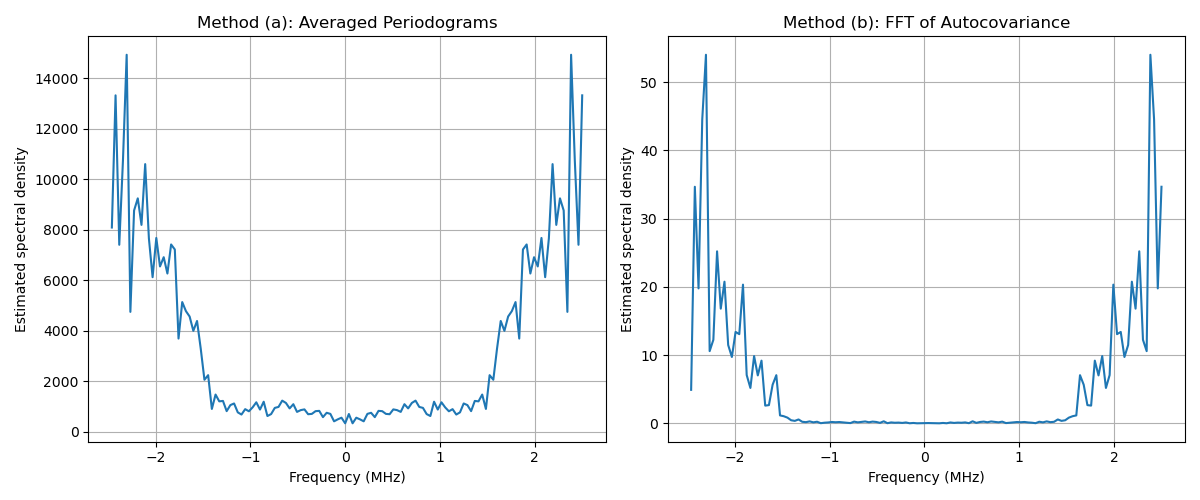
\includegraphics[width=0.8\textwidth]{./wss.png}
        \caption{Estimated spectral density $S_x$ using the two methods.}
        \label{fig:y_stats}
    \end{figure}
\end{document}